\chapter{Appendix to Chapter~\ref{ch:rss}}

\section{Sensor Placement Design Problem Statement}

We model the robot with discrete-time Dubins dynamics with three state variables ($q = [x, y, \theta]$), two control inputs for linear and angular velocity ($u = [v, \omega]$), and noisy transition model
\begin{align*}
    \mat{x \\ y \\ \theta}_{t+1} = \mat{x \\ y \\ \theta}_{t} + \mat{\Delta t v \cos(\theta + \Delta t \omega / 2) \\ \Delta t v \sin(\theta + \Delta t \omega / 2) \\ \Delta t \omega} + w_t
\end{align*}
where $\Delta t = 0.5$ and $w_t \in \R^3$ is the actuation noise ($w_t \sim \mathcal{N}(0, Q)$ with covariance $Q \in \R^{3\times3}$). The measurement model is
\begin{align*}
    z_t = \mat{(x_t - x_{b1})^2 + (y_t - y_{b1})^2 \\ (x_t - x_{b2})^2 + (y_t - y_{b2})^2 \\ \theta} + v_t
\end{align*}
where $v_t$ is the measurement noise ($v_t \sim \mathcal(0, R)$ and covariance $R \in \R^{3\times3}$), modeling range measurements from radio or acoustic beacons $b_1$ and $b_2$ and inertial or magnetic measurements of $\theta$. The initial state of the robot is normally distributed $q_0 \sim \mathcal{N}(\bar{q}_0, P_0)$ for mean initial state $\bar{q}_0 \in \R^3$ and initial covariance $P_0 \in \R^{3\times3}$. The navigation function (shown in Fig.~\ref{ch:rss:fig:agv_representative_trajectories}) is $V_t(x_t, y_t) = 2 (x_t^2 + y_t^2) + 0.05 / d_t$ ($d_t$ is the distance from the robot to the nearest obstacle at step $t$). Formally, we define this problem in the language of our framework in Table~\ref{ch:rss:tab:agv_design_problem}.

\begin{table}[tb]
    \renewcommand{\arraystretch}{1.5}
    \caption{Formal statement of the sensor placement design problem with $T$ discrete timesteps.}
    \label{ch:rss:tab:agv_design_problem}
    \begin{tabular}{|p{2.5cm}|p{14cm}|}
        \hline
        Design\ \ parameters & \begin{tabular}[c]{@{}l@{}}
                                   $\theta = [b_1, b_2, k] \in \R^6$ \\ Beacon locations: $b_i = (x_{bi}, y_{bi}) \in \R^2$ for $i=1,2$ \\
                                   Feedback gains: $k \in \R^2$
                               \end{tabular}                                                                                                                                                                                                                                                                                                                                                                                                                                             \\ \hline
        %
        Exogenous parameters & \begin{tabular}[c]{@{}l@{}}
                                   $\phi = [q_0, w_0, \ldots, w_{T-1}, v_0, \ldots, v_{T-1}] \in \R^{3 + 6T}$ \\ Initial state: $q_0 \in \R^3,\ q_0 \sim \mathcal{N}(\bar{q}_0, P_0)$;\\\phantom{Initial State: }$P_0 = 0.001 I_{3\times3}$\\ Actuation noise: $w_t \in \R^3,\ w_t\sim \mathcal{N}(0, Q)$;\\\phantom{Actuation noise: }$Q = (\Delta t)^2 \text{diag}\pn{[0.001, 0.001, 0.01]}$\\ Measurement noise: $v_t \in \R^3,\ v_t\sim \mathcal{N}(0, R)$\\\phantom{measurement noise: }$R = \text{diag}\pn{[0.1, 0.01, 0.01]}
                                   $\end{tabular} \\ \hline
        %
        Simulator            & $S$ initializes the robot with state $q_0$ and EKF state estimate $\bar{q}_0$ and error covariance $P_0$, then steps forward with interval $\Delta t = 0.5$ for $T = 60$ total steps. At each step, the simulator
        \begin{enumerate}
            \item Evaluates the navigation function to find a collision-free path to the goal,
            \item Uses a feedback controller to track that path,
            \item Updates the state using forward Euler integration,
            \item Performs an EKF prediction, obtains a measurement $z_t$, and performs an EKF update.
        \end{enumerate}

        $S$ returns a trace $s_t = [q, \hat{q}, P_{t|t}, V_t]$ containing true states, estimated states, estimated posterior error covariance, and the value of the navigation function at each time step.
        \\ \hline
        %
        Cost                 & $J$ has three components. The first ($\norm{q_t - \hat{q}_t}^2$) minimizes the estimation error of the EKF, the second ($\norm{q_t}$) guides the robot towards the goal, and the third (both $V_t$ terms) avoids collision with the environment:
        $J = \frac{1}{T} \sum_{t=1}^T \pn{100 \norm{q_t - \hat{q}_t}^2 + \norm{q_t}^2 + 0.1 V_t}$ $+ 0.1 \max_t V_t$
        \\ \hline
        %
        Constraints          & $(x_{bi}, y_{bi}) \in [-3, 0] \times [-1, 1]$ for $i=1, 2$                                                                                                                                                                                                                                                                                                                                                                                                                                                                                                                                     \\ \hline
    \end{tabular}
\end{table}

\section{Multi-agent Manipulation Design Problem Statement}

We model each ground robot as a double integrator with states $[p_x, p_y, \theta, v_x, v_y, \omega]$. Given control inputs representing desired linear velocity $v_d$ in the $[\cos\theta, \sin\theta]$ direction and desired angular velocity $\omega_d$, the robot tracks those desired velocities by applying forces and torques subject to a friction cone constraint. The box is modeled as a rigid body with friction against the ground. Contact forces between the box and each robot are modeled using a penalty method described in~\cite{suh2021_bundled_gradients}, where the normal force is given by $f_n = k_c \min(\phi, 0) - k_d \dot{\phi} \mathbbm{1}_{\phi < 0}$ ($\phi$ is the signed distance between the robot and the box, $k_c = \SI{300}{N/m}$ is the contact stiffness, $k_d$ is a damping coefficient chosen to ensure critical damping, and $\mathbbm{1}_{\phi < 0}$ is the indicator function equal to 1 when the box and robot are in contact and 0 otherwise). Friction in the box/ground and box/robot contacts was modeled as Coulomb friction, resulting in a tangential force $f_t = \mu f_n$ with $\mu = c\psi$ if $\psi < \psi_s$ and $\mu = \mu_d$ otherwise, where $mu_d$ is the coefficient of dynamic friction ($\mu_d$ varies for each contact pair), $\psi$ is the tangential velocity at the point of contact, $\psi_s = \SI{0.3}{m/s}$ is the tangential velocity where slipping begins, and $c = \mu_d / \psi_s$ was chosen to ensure a continuous friction model.

Each ground robot uses a proportional controller (with tunable gains) to find $v_d$ and $\omega_d$ to track a cubic spline reference trajectory. The start point of each spline is set to match the robot's current position, the end point is set based a known offset from the desired box location, and the central control point of the spline is set using a neural network (with tunable parameters). The neural network is given inputs including the current position of each robot and the desired box pose, all referenced against the current box pose, and it predicts $(x, y)$ locations for the control point for each robot. The network uses $\tanh$ activations on each hidden layer.

Formally, we define this problem in the language of our framework (design parameters, exogenous parameters, etc.) in Table~\ref{ch:rss:tab:mam_design_problem}. The design parameters include the trajectory tracking control gains and network parameters, while the exogenous parameters include the desired box pose, coefficients of friction, box mass, and initial robot poses.

\begin{table}[tb]
    \renewcommand{\arraystretch}{1.5}
    \caption{Formal statement of the collaborative manipulation design problem using a planning network with $n_p$ total parameters (weights and biases).}
    \label{ch:rss:tab:mam_design_problem}
    \begin{tabular}{|p{2.5cm}|p{14cm}|}
        \hline
        Design\ \ parameters & \begin{tabular}[c]{@{}l@{}}$\theta = [k_v, k_\omega, w_i, b_i] \in \R^{2 + n_p}$\\ Trajectory tracking gains: $[k_v, k_w] \in \R^2$\\ Network weights and biases: $(w_i, b_i)$ for $i=1,\ldots,n_p$\end{tabular}                                                                                                                                                                                                                                                                                                                                                                                                                                                                                                                                                             \\ \hline
        Exogenous parameters & \begin{tabular}[c]{@{}l@{}}$\phi = [\mu_{rg}, \mu_{bg}, \mu_{br}, m_b, p_{bd}, p_{r1}, p_{r2}] \in \R^{13}$  \\ Robot/ground, box/ground, box/robot coefficients of friction:\\\quad$[\mu_{rg}, \mu_{bg}, \mu_{br}] \in [0.6, 0.8] \times [0.4, 0.6] \times [0.1, 0.3]$ \\
                                   Box mass: $m_b \in [0.9, 1.1]$                                                                \\
                                   Desired box pose:                                                                             \\\quad $p_{bd} = [x_d, y_d, \theta_d] \in [0, 0.5]^2 \times [-\pi/4, \pi/4]$ \\ (Above parameters are uniformly distributed) \\
                                   Initial robot pose: $p_{ri} = [x_{0}, y_0, \theta_0] \sim \mathcal{N}(\bar{p}_{ri}, \Sigma)$; \\\quad $\Sigma = 0.01 I_{3\times3}$, $i=1,2$.\end{tabular}                                                                                                                                                                                                                                                                                                                                                                                 \\ \hline
        Simulator            & $S$ initializes the robots at the initial states in $\phi$ relative to the box. Since these initial states may be in contact, we simulate \SI{0.5}{s} of settling time at a \SI{0.01}{s} timestep, then re-index the robot positions and desired box pose relative to the settled box pose. We then evaluate the planning network and track the planned path for \SI{4}{s} at a \SI{0.01}{s} timestep. At each timestep, 1) evaluate the spline tracking controller, 2) evaluate contact dynamics between the box, robots, and ground, and 3) integrate forces and torques to obtain box and robot states at the next timestep. $S$ returns a trace $s_t = [q_{r1}, q_{r2}, q_{b}]$ containing the states of each robot and the box over time (relative to the initial pose of the box after the settling period). \\ \hline
        Cost                 & $J$ is simply the squared distance between the final box pose and the desired box position $(x - x_d)^2 + (y - y_d)^2 + (\theta - \theta_d)^2$                                                                                                                                                                                                                                                                                                                                                                                                                                                                                                                                                                                                                                                                     \\ \hline
        Constraints          & Network parameters were not constrained. $k_v$ and $k_w$ were constrained to be less than 10.                                                                                                                                                                                                                                                                                                                                                                                                                                                                                                                                                                                                                                                                                                                      \\ \hline
    \end{tabular}
\end{table}

\begin{figure*}[t]
    \centering
    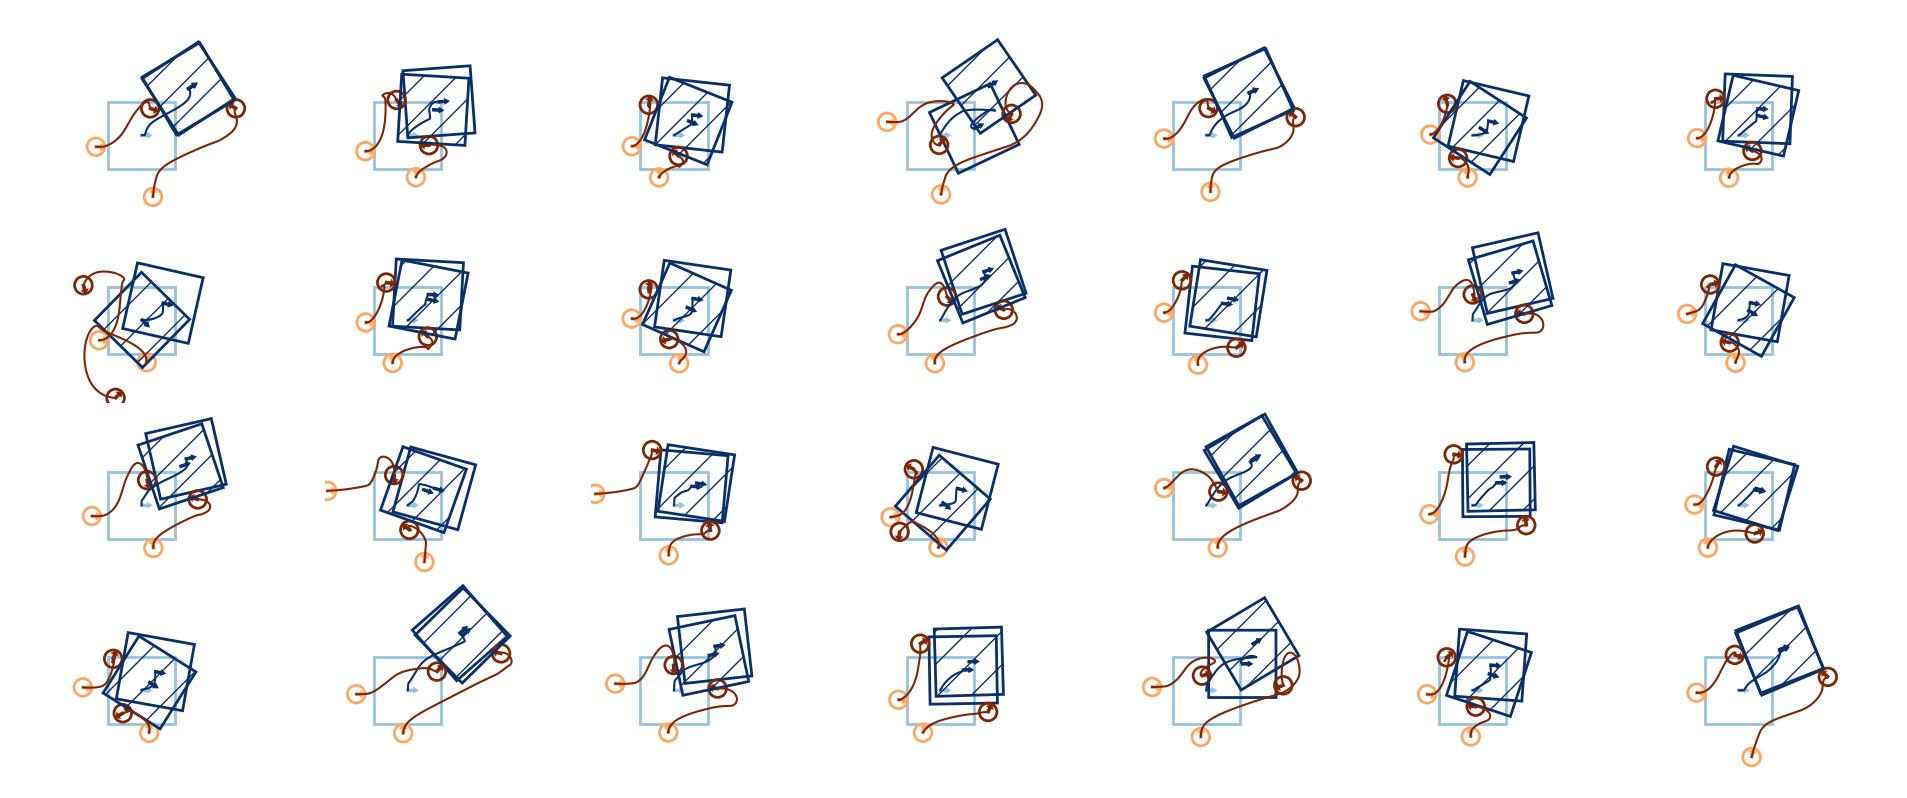
\includegraphics[width=\linewidth]{rss/mam_more.png}
    \caption{Additional examples of optimized multi-agent manipulation behavior in simulation, showing that the optimized strategy reaches the goal in most cases. Each example shows the results of executing the optimized pushing strategy for \SI{4}{s} with a randomly selected set of friction coefficients, random target pose, and random initial robot poses. Light/dark colors indicate initial/final positions, respectively, and the striped box indicates the target pose.}
    \label{ch:rss:fig:mam_more}
\end{figure*}

\section{Kolmogorov-Smirnov Test Results}

Table~\ref{ch:rss:tab:ks_test_agv} provides results from one-sided KS tests for the GEVD estimated using Algorithm~\ref{ch:rss:alg:worst_case_cost} in the sensor placement case study, while Table~\ref{ch:rss:tab:ks_test_mam} provides similar results for Algorithm~\ref{ch:rss:alg:sensitivity} in the collaborative manipulation case study.

\begin{table*}[thb]
    \renewcommand{\arraystretch}{1.5}
    \centering
    \begin{tabular}{r||p{4cm}|c|c|p{5cm}}
                     & Null Hypothesis                                & \shortstack{KS                                                                                     \\ Statistic} & p-value & Conclusion ($p < 0.05$)                                                   \\ \hline\hline
        \shortstack{False                                                                                                                                                  \\Optimism} & 97\% GEVD under-estimates worst-case performance & 0.0410         & 0.0337  & Reject; 97\% GEVD \textit{does not} under-estimate worst-case performance \\ \hline
        Conservatism & 3\% GEVD over-estimates worst-case performance & 0.0529         & 0.00354 & Reject; 3\% GEVD \textit{does not} over-estimate worst-case performance
    \end{tabular}
    \caption{Results of one-sided KS tests for the sensor placement case study. These results indicate that Algorithm~\ref{ch:rss:alg:worst_case_cost} is sound in this case.}\label{ch:rss:tab:ks_test_agv}
\end{table*}

\begin{table*}[thb]
    \renewcommand{\arraystretch}{1.5}
    \centering
    \begin{tabular}{r||p{4cm}|c|c|p{5cm}}
                     & Null Hypothesis                     & \shortstack{KS                                                                                       \\ Statistic} & p-value              & Conclusion ($p < 0.05$)                                        \\ \hline\hline
        \shortstack{False                                                                                                                                         \\Optimism} & 97\% GEVD under-estimates sensitivity & 0.0399         & $6.75\times10^{-5}$  & Reject; 97\% GEVD \textit{does not} under-estimate sensitivity \\ \hline
        Conservatism & 3\% GEVD over-estimates sensitivity & 0.0618         & $1.03\times10^{-10}$ & Reject; 3\% GEVD \textit{does not} over-estimate sensitivity
    \end{tabular}
    \caption{Results of one-sided KS tests for the collaborative manipulation case study. These results indicate that Algorithm~\ref{ch:rss:alg:sensitivity} is sound in this case.}\label{ch:rss:tab:ks_test_mam}
\end{table*}